\section{End-to-end feasible proxies for DCOPF}
\label{sec:layers}

    % \mt{There is a clear connection between our feasibility layers and the simplex algorithm. The way we are increasing/decreasing energy dispatch is exactly what simplex pivots would be doing (except we move multiple generators at the same time).}
    % \mt{Additional questions on the methodology:\\
    % * What about two categories of reserve?\\
    % * Can we do a weighted proportional response? (so that we increase the dispatch of cheap generators more than we increase that of expensive generators)}

This section presents the Economic Dispatch (ED) formulation
considered in the paper, and introduces new repair layers for power
balance and reserve requirement constraints.  The repair layers are
computationally efficient and differentiable: they can be implemented
in standard machine-learning libraries, enabling end-to-end feasible
optimization proxies.
% Because of space limitations, all proofs are deferred to Appendix \ref{app:proofs}.

\subsection{Problem Formulation}
\label{sec:DCOPF}
    
The paper considers an ED formulation with reserve requirements. It
is modeled as a linear program of the form
    \begin{subequations}
    \label{eq:DCOPF}
    \begin{align}
        \min_{\pg, \res, \xith} \quad & c(\pg) + \Mth \| \xith \|_{1}\\
        \text{s.t.} \quad
            & \mathbf{e}^{\top} \pg = \mathbf{e}^{\top} \pd, \label{eq:DCOPF:power_balance}\\
            & \mathbf{e}^{\top} \res \geq R, \label{eq:DCOPF:reserve_requirements}\\
            & \pg + \res \leq \pgmax,  \label{eq:DCOPF:eco_max}\\
            & \mathbf{0} \leq \pg \leq \pgmax, \label{eq:DCOPF:dispatch_bounds}\\
            & \mathbf{0} \leq \res \leq \resmax, \label{eq:DCOPF:reserve_bounds}\\
            & \mathbf{\ubar{f}} -\xith \leq \Phi (\pg - \pd)  \leq \mathbf{\bar{f}} +\xith, \label{eq:DCOPF:PTDF}\\
            & \xith \geq \mathbf{0}.  \label{eq:DCOPF:thermal_slack_positive}
    \end{align}
    \end{subequations}

Constraints \eqref{eq:DCOPF:power_balance} and
\eqref{eq:DCOPF:reserve_requirements} are the global power balance and
minimum reserve requirement constraints, respectively.  Constraints
\eqref{eq:DCOPF:eco_max} ensure that each generator reserves can be
deployed without violating their maximum capacities.  Constraints
\eqref{eq:DCOPF:dispatch_bounds} and \eqref{eq:DCOPF:reserve_bounds}
enforce minimum and maximum limits on each generator energy and
reserve dispatch.  Without loss of generality, the paper assumes that
each bus has exactly one generator, each generator minimum output is
zero, and $\bar{r}_{g} \leq \bar{p}_{g}, \forall g$. Constraints
\eqref{eq:DCOPF:PTDF} express the thermal constraints on each branch using
a Power Transfer Distribution Factor (PTDF) representation.  In this
paper, the thermal constraints are soft constraints, i.e., they can be
violated but doing so incurs a (high) cost.  This is modeled via
artificial slack variables $\xith$ which are penalized in the
objective.  Treating thermal constraints as soft is in line with
economic dispatch formulations used by system operators to clear
electricity markets in the US \cite{Ma2009_MISO_SCED,BPM002_D}.  The
PTDF-based formulation is also the state-of-the-art approach used in
industry \cite{Ma2009_MISO_SCED,Holzer2022_MISO_SFT}.  In typical
operations, only a small number of these constraints are active at the
optimum.  Therefore, efficient implementations add thermal constraints
\eqref{eq:DCOPF:PTDF} lazily.

The hard constraints in Problem \eqref{eq:DCOPF} are the bounds on
energy and reserve dispatch, the maximum output, the power balance
\eqref{eq:DCOPF:power_balance} and the reserve requirements
\eqref{eq:DCOPF:reserve_requirements}.  Note that bounds on individual
variables can easily be enforced in a DNN architecture e.g., via
clamping or sigmoid activation. However, it is not trivial to
\emph{simultaneously} satisfy variable bounds, power balance and
reserve requirements.  To address this issue, the rest of this section
introduces new, computationally efficient repair layers.

\subsection{The Power Balance Repair Layer}
\label{sec:layers:power_balance}

    \newcommand{\hypercube}{\mathcal{H}}
    \newcommand{\hypersimplex}[1]{\mathcal{S}_{#1}}
    \newcommand{\etaup}{\eta^{\uparrow}}
    \newcommand{\etadn}{\eta^{\downarrow}}

The proposed power balance repair layer takes as input an initial
dispatch vector $\pg$, which is assumed to satisfy the min/max
generation bounds \eqref{eq:DCOPF:dispatch_bounds}, and outputs a
dispatch vector $\tilde{\pg}$ that satisfies constraints
\eqref{eq:DCOPF:dispatch_bounds} and \eqref{eq:DCOPF:power_balance}.
Formally, let $D \, {=} \, \mathbf{e}^{\top} \pd$, and denote by
$\hypercube$ and $\hypersimplex{D}$ the following hypercube and
hypersimplex
    \begin{align}
        \label{eq:layers:hypercube}
        \hypercube &= \left\{
            \pg \in \mathbb{R}^{n}
        \ \middle| \ 
            \mathbf{0} \leq \pg \leq \mathbf{\bar{p}}
        \right\},\\
        \label{eq:layers:hypersimplex}
        \hypersimplex{D} &= \left\{
            \pg \in \mathbb{R}^{n}
        \ \middle| \ 
            \mathbf{0} \leq \pg \leq \mathbf{\bar{p}}, \ 
            \mathbf{e}^{\top} \pg = D
        \right\}.
    \end{align}

\noindent
Note that $\hypercube$ is the feasible set of constraints
\eqref{eq:DCOPF:dispatch_bounds}, while $\hypersimplex{D}$ is the
feasible set of constraints \eqref{eq:DCOPF:power_balance} and
\eqref{eq:DCOPF:dispatch_bounds}. The proposed power balance repair
layer, denoted by $\mathcal{P}$, is given by
    \begin{align}
        \label{eq:power_balance_layer}
        \begin{array}{rl}
            % \mathcal{P}: \quad
            % \hypercube & \longrightarrow \quad \hypersimplex{D}\\
            \mathcal{P}(\pg) & = \left\{
            \begin{array}{ll}
                (1 - \etaup) \pg + \etaup \mathbf{\bar{p}} &  \text{if } \mathbf{e}^{\top} \pg < D\\
                (1 - \etadn) \pg + \etadn \mathbf{0}  &  \text{if } \mathbf{e}^{\top} \pg \geq D
            \end{array}
        \right.
        \end{array}
    \end{align}
    where $\pg \, {\in} \, \mathcal{H}$, and $\etaup$, $\etadn$ are defined as follows:
    \begin{align}
        \label{eq:power_balance_layer:ratios}
        \etaup   &= \frac{\mathbf{e}^{\top}\pd - \mathbf{e}^{\top} \pg}{\mathbf{e}^{\top} \mathbf{\bar{p}} - \mathbf{e}^{\top}\pg}, &
        \etadn &= \frac{\mathbf{e}^{\top}\pg - \mathbf{e}^{\top}\pd}{\mathbf{e}^{\top} \pg - \mathbf{e}^{\top} \mathbf{0}}.
    \end{align}
    Theorem \ref{thm:power_balance_layer} below shows that $\mathcal{P}$ is well-defined.

\begin{theorem}
    \label{thm:power_balance_layer}
    Assume that $0 < \mathbf{e}^{\top} \pd = D < \mathbf{e}^{\top} \pgmax$ and $\pg \in \hypercube$.\\
    Then, $\mathcal{P}(\pg) \in \hypersimplex{D}$.
\end{theorem}
\begin{proof}
Let $\mathbf{\tilde{p}} \, {=} \, \mathcal{P}(\pg)$, and assume $\mathbf{e}^{\top} \pg \, {<} \, D$; the case $\mathbf{e}^{\top} \pg \, {\geq} \, D$ is treated similary.
It follows that $\etaup \, {\in} \, [0, 1]$, i.e., $\mathbf{\tilde{p}}$ is a convex
combination of $\pg$ and $\pgmax$.
Thus, $\mathbf{\tilde{p}} \in
\hypercube$.  Then,
    \begin{align*}
        \mathbf{e}^{\top}\mathbf{\tilde{p}}
        &= (1 - \etaup) \mathbf{e}^{\top}\pg + \etaup \mathbf{e}^{\top}\bar{\pg}\\
        &= \etaup(\mathbf{e}^{\top}\bar{\pg} - \mathbf{e}^{\top}\pg) + \mathbf{e}^{\top} \pg\\
        &= \frac{D - \mathbf{e}^{\top} \pg}{\mathbf{e}^{\top} \mathbf{\bar{p}} - \mathbf{e}^{\top}\pg} (\mathbf{e}^{\top}\bar{\pg} - \mathbf{e}^{\top}\pg) + \mathbf{e}^{\top} \pg\\
        &= D - \mathbf{e}^{\top}\pg + \mathbf{e}^{\top} \pg = D.
    \end{align*}
    Thus, $\mathbf{\tilde{p}}$ satisfies the power balance and $\mathbf{\tilde{p}} \in \hypersimplex{D}$.
    % Similarly, assume $\mathbf{e}^{\top}\pg \geq D$.
    % Then
    % \begin{align*}
    %     \mathbf{e}^{\top}\mathbf{\tilde{p}}
    %     &= (1 - \etadn) \mathbf{e}^{\top}\pg + \etadn \mathbf{e}^{\top}\mathbf{0}\\
    %     &= (1 - \frac{\mathbf{e}^{\top}\pg - D}{\mathbf{e}^{\top} \pg}) \mathbf{e}^{\top}\pg = D,
    % \end{align*}
    % which concludes the proof.
\end{proof}

Note that feasible predictions are not modified: if $\pg \in
\hypersimplex{D}$, then $\mathcal{P}(\pg) = \pg$. The edge cases not
covered by Theorem \ref{thm:power_balance_layer} are handled as
follows.  When $D \leq 0$ (resp. $D \geq \mathbf{e}^{\top} \pgmax$),
each generator is set to its lower (resp. upper) bound; this can be
achieved by clamping $\etaup$ (resp. $\etadn$) to $[0, 1]$. 
If these inequalities are strict, Problem \eqref{eq:DCOPF} is
trivially infeasible, and $\mathcal{P}(\pg)$ is the solution that
minimizes power balance violations.

The power balance layer is illustrated in Figure
\ref{fig:feasibility_layer:hypersimplex}, for a two-generator system.
The layer has an intuitive interpretation as a proportional response
mechanism.  Indeed, if the initial dispatch $\pg$ has an energy
shortage, i.e., $\mathbf{e}^{\top} \pg \, {<} \, D$, the output of
each generator is increased by a fraction $\etaup$ of its upwards
headroom.  Likewise, if the initial dispatch has an energy surplus,
i.e., $\mathbf{e}^{\top} \pg \, {>} \, D$, the output of each
generator is decreased by a fraction $\etadn$ of it downwards
headroom.

\begin{figure}[!t]
        \centering
        \resizebox{0.48\columnwidth}{!}{
        \begin{tikzpicture}[x=2cm,y=2cm]
            % X Axis
            \draw[black,-stealth] (-0.1, 0.0) -- (1.25, 0.0);
            \node[below] at (1.25, 0.0) {\footnotesize $p_{1}$};
            % Y axis
            \draw[black,-stealth] (0.0, -0.1) -- (0.0, 1.25);
            \node[left] at (0.0, 1.25) {\footnotesize $p_{2}$};
            
            % Unit hypercube
            \draw[black] (0,0) -- (0, 1) -- (1,1) -- (1,0) -- cycle;
            
            % More visuals for radial projection
            % \draw[gray, opacity=0.2] (1,1) -- (0.00, 0.66);
            % \draw[gray, opacity=0.2] (1,1) -- (0.00, 0.33);
            % \draw[gray, opacity=0.2] (1,1) -- (0.00, 0.00);
            % \draw[gray, opacity=0.2] (1,1) -- (0.33, 0.00);
            % \draw[gray, opacity=0.2] (1,1) -- (0.66, 0.00);
            
            % Power balance constraint
            \draw[red,line width=1pt] (0.1, 1.1) -- (1.1, 0.1);
            \node[right, color=red] at (0.1, 1.2) {\footnotesize $\mathbf{e}^{\top}\pg = D$};
            
            % Max output
            \node[draw=blue, fill=blue, inner sep=0pt,minimum size=3pt] (p_bar) at (1.00, 1.00) {};
            % \node[above right] at (1,1) {\tiny $(1, 1)$};
            % Prediction
            \node[diamond,draw=blue, fill=blue, inner sep=0pt,minimum size=3pt] (p_hat) at (0.30, 0.30) {};
            \node[left] at (0.3, 0.3) {\footnotesize $\pg$};
            % Feasible point
            \node[circle,draw=blue, fill=blue, inner sep=0pt,minimum size=3pt] (p_til) at (0.6, 0.6) {};
            \node[right] at (0.65, 0.6) {\footnotesize $\mathbf{{\tilde{p}}}$};
            
            % Proportional response visual
            \draw[black,-stealth] (p_hat) -- (p_til);
            \draw[black,densely dotted] (p_til) -- (p_bar);
        \end{tikzpicture}}
        \hfill
        \resizebox{0.48\columnwidth}{!}{
        \begin{tikzpicture}[x=2cm,y=2cm]
            % X Axis
            \draw[black,-stealth] (-0.1, 0.0) -- (1.25, 0.0);
            \node[below] at (1.25, 0.0) {\footnotesize $p_{1}$};
            % Y axis
            \draw[black,-stealth] (0.0, -0.1) -- (0.0, 1.25);
            \node[left] at (0.0, 1.25) {\footnotesize $p_{2}$};
            
            % Unit hypercube
            \draw[black] (0,0) -- (0, 1) -- (1,1) -- (1,0) -- cycle;
            
            % More visuals for radial projection
            % \draw[gray, opacity=0.2] (0,0) -- (1.00, 0.66);
            % \draw[gray, opacity=0.2] (0,0) -- (1.00, 0.33);
            % \draw[gray, opacity=0.2] (0,0) -- (1.00, 1.00);
            % \draw[gray, opacity=0.2] (0,0) -- (0.33, 1.00);
            % \draw[gray, opacity=0.2] (0,0) -- (0.66, 1.00);
            
            % Power balance constraint
            \draw[red,line width=1pt] (0.1, 1.1) -- (1.1, 0.1);
            \node[right, color=red] at (0.1, 1.2) {\footnotesize $\mathbf{e}^{\top}\pg = D$};
            
            % Min output
            \node[draw=blue, fill=blue, inner sep=0pt,minimum size=3pt] (p_bar) at (0.00, 0.00) {};
            % \node[above left] at (0,0) {\footnotesize $(0,0)$};
            % Prediction
            \node[diamond,draw=blue, fill=blue, inner sep=0pt,minimum size=3pt] (p_hat) at (0.80, 0.80) {};
            \node[right] at (0.8, 0.8) {\footnotesize $\pg$};
            % Feasible point
            \node[circle,draw=blue, fill=blue, inner sep=0pt,minimum size=3pt] (p_til) at (0.6, 0.6) {};
            \node[left] at (0.58, 0.58) {\footnotesize $\mathbf{{\tilde{p}}}$};
            
            % Proportional response visual
            \draw[black,-stealth] (p_hat) -- (p_til);
            \draw[black,densely dotted] (p_til) -- (p_bar);
        \end{tikzpicture}}
        \hfill\\
        \caption{%
            Illustration of the power balance layer with input $\pg$ and output $\mathbf{\tilde{p}}$.
            Left: $\mathbf{e}^{\top}\pg \, {<} \, D$ (energy shortage) and generators' dispatches are increased.
            Right: $\mathbf{e}^{\top}\pg \, {>} \, D$ (energy surplus) and generators' dispatches are decreased.
        }
        \label{fig:feasibility_layer:hypersimplex}
\end{figure}

Note that $\hypersimplex{D}$ is defined by the combination of bound
constraints and one equality constraint.  Other works such as
\cite{donti2021dc3,Li2022_LOOP-LC} handle the latter via equality
completion.  While this approach satisfies the equality constraint by
design, the recovered solution is not guaranteed to satisfy min/max
bounds, and may fail to do so in general.  In contrast, under the only
assumption that $\pg \in \hypercube$, the proposed layer
\eqref{eq:power_balance_layer} jointly enforces \emph{both}
constraints, thus alleviating the need for the gradient unrolling of
\cite{donti2021dc3} or gauge mapping of \cite{Li2022_LOOP-LC}.
Finally, the proposed layer generalizes to hypersimplices of the form
    \begin{align}
        \label{eq:power_balance_layer:hypersimplex:general}
        \left\{
            x \in \mathbb{R}^{n}
        \ \middle| \ 
            l \leq x \leq u, a^{T}x = b
        \right\},
    \end{align}
    where $a \in \mathbb{R}^{n}, b \in \mathbb{R}$ and $l \leq u \in \mathbb{R}^{n}$ are finite bounds.

\subsection{The Reserve Repair Layer}
\label{sec:layers:reserve}

This section presents the proposed reserve feasibility layer, which
ensures feasibility with respect to constraints
\eqref{eq:DCOPF:reserve_requirements}, \eqref{eq:DCOPF:eco_max}, and
\eqref{eq:DCOPF:reserve_bounds}.  The approach first builds a compact
representation of these constraints by projecting out the reserve
variables $\res$.  This makes it possible to consider only the $\pg$
variables, which in turn enables a computationally efficient and
interpretable feasibility restoration. Let $\pg \in \hypersimplex{D}$
be fixed, and consider the problem of maximizing total reserves, which
reads
    \begin{subequations}
    \label{eq:ReserveRecovery}
    \begin{align}
        % \mathcal{R}(\pg) \quad 
        \max_{\mathbf{r}} \quad & \mathbf{e}^{\top} \mathbf{r} \label{eq:ReserveRecovery:obj}\\
        \text{s.t.} \quad & \mathbf{r} \leq \bar{\pg} - \pg, \label{eq:ReserveRecovery:eco_max}\\
        & 0 \leq \mathbf{r} \leq \bar{\mathbf{r}}. \label{eq:ReserveRecovery:reserve_bounds}
    \end{align}
    \end{subequations}
    Since $\pg$ is fixed, constraints \eqref{eq:ReserveRecovery:eco_max}--\eqref{eq:ReserveRecovery:reserve_bounds} reduce to simple variable bounds on the $\mathbf{r}$ variables.
    It then immediately follows that the optimal solution to Problem \eqref{eq:ReserveRecovery} is given by
    \begin{align}
        \label{eq:reserve_recovery:optimal_reserves}
        r^{*}_{g} = \min\{\bar{r}_{g}, \bar{p}_{g} - p_{g} \}, \ \forall g.
    \end{align}
    This observation is used to project out the reserve variables as stated in Lemma \ref{lem:reserve_layer:compact_representation} below.

\begin{lemma}
\label{lem:reserve_layer:compact_representation}
Let $\pg \in \hypersimplex{D}$. There exists reserves $\mathbf{r}$ such that $(\pg, \mathbf{r})$ is feasible for Problem \eqref{eq:DCOPF} if and only if
\begin{align}
\label{eq:reserves:sufficient}
\sum_{g} \min\{\bar{r}_{g}, \bar{p}_{g} - p_{g} \} \geq R.
\end{align}
\end{lemma}
\begin{proof}
The proof follows from the fact that $(\pg, \mathbf{r})$ is feasible
for Problem \eqref{eq:DCOPF} if and only if Problem
\eqref{eq:ReserveRecovery} has an objective value not smaller than
$R$. Substituting the optimal solution given in
Eq. \eqref{eq:reserve_recovery:optimal_reserves}, this last statement
is exactly equivalent to $\sum_{g} \min\{\bar{r}_{g}, \bar{p}_{g} -
p_{g} \} \geq R$.
\end{proof}
    
The proposed reserve repair layer builds on the power balance repair
layer of Section \ref{sec:layers:power_balance}, and on the compact
formulation of Eq. \eqref{eq:reserves:sufficient}.  Namely, it takes
as input $\pg \, {\in} \, \hypersimplex{D}$, and outputs
$\mathcal{R}(\pg) \, {\in} \, \hypersimplex{D}$ that satisfies
Eq. \eqref{eq:reserves:sufficient}.  Given $\mathcal{R}(\pg)$, reserve
variables can be recovered in $O(|\mathcal{G}|)$ time using
Eq. \eqref{eq:reserve_recovery:optimal_reserves}.

The reserve repair layer is presented in Algorithm
\ref{alg:FFR:reserves}.  First, a tentative reserve allocation is
computed using Eq. \ref{eq:reserve_recovery:optimal_reserves}, and the
corresponding reserve shortage $\Delta_{R}$ is computed.  Then,
generators are split into two groups $G^{\uparrow}$ and
$\mathcal{G}^{\downarrow}$.  Generators in $\mathcal{G}^{\uparrow}$
are those for which constraint \eqref{eq:DCOPF:reserve_bounds} is
active: their dispatch can be increased without having to reduce their
reserves.  Generators in $\mathcal{G}^{\downarrow}$ are those for
which constraint \eqref{eq:DCOPF:eco_max} is active: one must reduce
their energy dispatch to increase their reserves.  Then, the algorithm
computes the maximum possible increase ($\Delta^{\uparrow}$) and
decrease ($\Delta^{\downarrow})$ in energy dispatch for the two
groups.  Finally, each generator energy dispatch is increased
(resp. decreased) proportionately to its increase (resp. decrease)
potential so as to meet total reserve requirements.  The total
increase in energy dispatch is equal to the total decrease, so that
power balance is always maintained.
    
\begin{algorithm}[!t]
        \caption{Reserve Repair Layer}
        \label{alg:FFR:reserves}
        \begin{algorithmic}[1]
            \REQUIRE Initial prediction $\pg \in \hypersimplex{D}$, maximum limits $\mathbf{\bar{p}}, \mathbf{\bar{r}}$, reserve requirement $R$
            \STATE $\Delta_{R} \gets R - \sum_{g} \min \{ \bar{r}_{g}, \bar{p}_{g} - p_{g} \}$
            \STATE $\mathcal{G}^{\uparrow} \gets \left\{ g \ \middle| \ p_{g} \leq \bar{p}_{g} - \bar{r}_{g} \right\}$
            \STATE $\mathcal{G}^{\downarrow} \gets \left\{ g \ \middle| \  p_{g} > \bar{p}_{g} - \bar{r}_{g} \right\}$
            \STATE $\Delta^{\uparrow} \gets \sum_{g \in \mathcal{G}^{\uparrow}} (\bar{p}_{g} - \bar{r}_{g}) - p_{g}$
            \STATE $\Delta^{\downarrow} \gets \sum_{g \in \mathcal{G}^{\downarrow}} p_{g} - (\bar{p}_{g} - \bar{r}_{g})$
            \STATE $\Delta \gets \max(0, \min(\Delta_{R}, \Delta^{\uparrow}, \Delta^{\downarrow}))$
            \STATE $\alpha^{\uparrow} \gets \Delta / \Delta^{\uparrow}$, $\alpha^{\downarrow} \gets \Delta / \Delta^{\downarrow}$, \label{alg:FFR:proportional_response_weigths}
            \STATE Energy dispatch adjustment
                \begin{align*}
                    \tilde{p}_{g} &= \left\{
                        \begin{array}{ll}
                            (1 - \alpha^{\uparrow}) p_{g} + \alpha^{\uparrow} (\bar{p}_{g} - \bar{r}_{g}) & \forall g \in \mathcal{G}^{\uparrow} \\
                            (1 - \alpha^{\downarrow}) p_{g} + \alpha^{\downarrow} (\bar{p}_{g} - \bar{r}_{g}) & \forall g \in \mathcal{G}^{\downarrow}
                        \end{array}
                    \right.
                \end{align*}
                \label{alg:FFR:proportional_response}
            \STATE \textbf{return} $\mathcal{R}(\pg) = \mathbf{\tilde{p}}$
        \end{algorithmic}
    \end{algorithm}

The reserve feasibility recovery is illustrated in Figure
\ref{fig:feasibility_recovery:reserve} for a two-generator system.
While it is easy to verify that $\mathcal{R}(\pg) \in
\hypersimplex{D}$, it is less clear whether $\mathcal{R}(\pg)$
satisfies Eq. \eqref{eq:reserves:sufficient}.  Theorem
\ref{thm:reserve_layer:guaranteed_feasibility} provides the
theoretical guarantee that either $\mathcal{R}(\pg)$ satisfies
Eq. \eqref{eq:reserves:sufficient}, or no feasible solution to Problem
\eqref{eq:DCOPF} exists.  Because of space limitations, the proof is
given in \cite{Chen2023_E2ELR_arxiv}.

\begin{theorem}
        \label{thm:reserve_layer:guaranteed_feasibility}
        Let $\pg \in \hypersimplex{D}$.
        Then, $\mathcal{R}(\pg) \in \hypersimplex{D}$.
        Furthermore, $\mathcal{R}(\pg)$ satisfies Eq. \eqref{eq:reserves:sufficient} if and only if Problem \eqref{eq:DCOPF} is feasible.
\end{theorem}

Theorem \ref{thm:reserve_layer:guaranteed_feasibility} also provides a
fast proof of (in)feasibility for Problem \eqref{eq:DCOPF}: it
suffices to evaluate $\mathcal{R}(\pg)$ for any $\pg \in
\hypersimplex{D}$ and check Eq. \eqref{eq:reserves:sufficient}.  This
can have applications beyond optimization proxies, e.g., to quickly
evaluate a large number of scenarios for potential reserve violations.
\revision{}{Finally, note that the results of Theorems \ref{thm:power_balance_layer} and \ref{thm:reserve_layer:guaranteed_feasibility} hold for any value of the maximum limits $\pgmax, \bar{\mathbf{r}}$ and reserve requirement $R$.}
    
    \begin{figure}[!t]
        \centering
        \resizebox{0.9\columnwidth}{!}{
        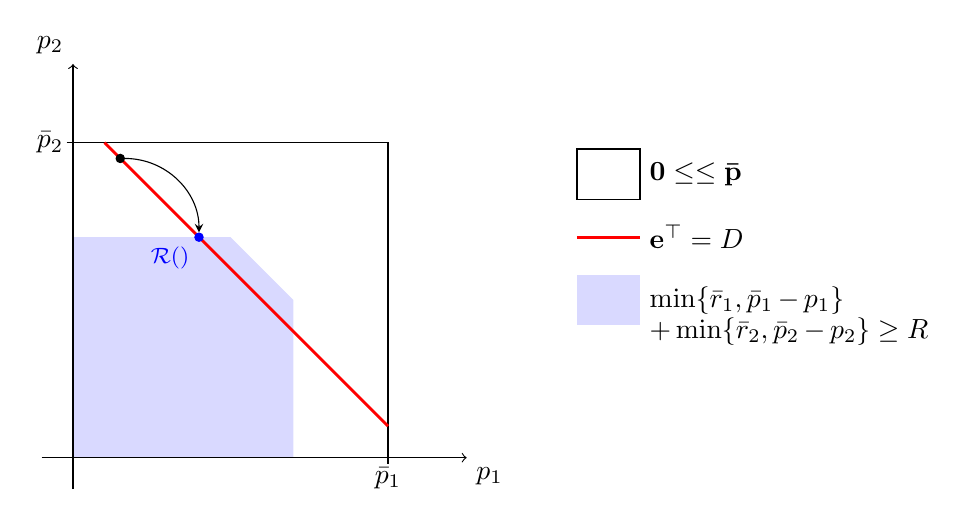
\begin{tikzpicture}[x=4cm,y=4cm]
            % X Axis
            \draw[black,->] (-0.1, 0.0) -- (1.25, 0.0);
            \node[below right] at (1.25, 0.0) {$p_{1}$};
                % EcoMin & EcoMax
                % \draw[black] (0, -0.27) -- (0, -0.23);
                % \node[below] at (0, -0.25) {$\ubar{p}_{1}$};
                \draw[black] (1, -0.02) -- (1, 0.02);
                \node[below] at (1, 0.0) {$\bar{p}_{1}$};
                % Reserve capacity
                % \draw[black] (0.6, -0.27) -- (0.6, -0.23);
                % \draw[black,<->] (0.6, -0.4) -- (1.0, -0.4);
                % \node[below] at (0.8, -0.4) {$\bar{r}_{1}$};
            
            % Y axis
            \draw[black,->] (0.0, -0.1) -- (0.0, 1.25);
            \node[above left] at (0.0, 1.25) {$p_{2}$};
                % EcoMin & EcoMax
                % \draw[black] (-0.02, 0) -- (0.02, 0);
                % \node[left] at (0, 0) {$\ubar{p}_{2}$};
                \draw[black] (-0.02, 1) -- (+0.02, 1);
                \node[left] at (0, 1) {$\bar{p}_{2}$};
                % Ecomax - reserve
                % \draw[black] (-0.27, 0.7) -- (-0.23, 0.7);
                % \draw[black,<->] (-0.4, 0.7) -- (-0.4, 1.0);
                % \node[left] at (-0.4, 0.85) {$\bar{r}_{2}$};
                
            % Reserve feasibility domain
            \fill[blue!50!white, fill opacity=0.3] (0,0) -- (0,0.7) -- (0.5, 0.7) -- (0.7, 0.5) -- (0.7, 0.0) -- cycle;
            
            % Domain of p1, p2
            \draw[black] (0,0) -- (0, 1) -- (1,1) -- (1,0) -- cycle;
            
            % Power balance constraint
            \draw[red,line width=1pt] (0.1, 1.0) -- (1.0, 0.1);
            % \draw[red,line width=1pt] (0.4, 0.8) -- (0.7, 0.5);
            
            % Infeasible prediction
            \node[circle,draw=black, fill=black, inner sep=0pt,minimum size=3pt] (phat_a) at (0.15, 0.95) {};
            \node[below left] at (0.15, 0.95) {\footnotesize $\pg$};
            % \node[circle,draw=black, fill=black, inner sep=0pt,minimum size=3pt] (phat_b) at (0.6, 0.6) {};
            % \node[circle,draw=black, fill=black, inner sep=0pt,minimum size=3pt] (phat_c) at (0.85, 0.35) {};
            
            % Feasible points of interest
            \node[circle,draw=blue, fill=blue, inner sep=0pt,minimum size=3pt] (pfeas1) at (0.4, 0.7) {};
            \node[below left, blue] at (0.4, 0.7) {\footnotesize $\mathcal{R}(\pg)$};
            % \node[circle,draw=blue, fill=blue, inner sep=0pt,minimum size=3pt] (pfeas2) at (0.7, 0.5) {};
            
            \draw[-stealth] (phat_a.east) to [out=0,in=90] (pfeas1.north);
            % \draw[-stealth] (phat_c.north) to [out=90,in=0] (pfeas2.east);
            
            % Legend
                % Domain of pg
                \draw[black] (1.6, 0.98) -- (1.8, 0.98) -- (1.8, 0.82) -- (1.6, 0.82) -- cycle;
                \node[right] at (1.8, 0.9) {$\mathbf{0} \leq \pg \leq \mathbf{\bar{p}}$};
                % Power Balance
                \draw[red, line width=1pt] (1.6, 0.7) -- (1.8, 0.7);
                \node[right] at (1.8, 0.7) {$\mathbf{e}^{\top} \pg = D$};
                % Reserve feasibility
                \fill[blue!50!white, fill opacity=0.3] (1.6, 0.58) -- (1.8, 0.58) -- (1.8, 0.42) -- (1.6, 0.42) -- cycle;
                \node[right] at (1.8, 0.5) {$\min\{\bar{r}_{1}, \bar{p}_{1} \, {-} \, p_{1}\}$};
                \node[right] at (1.8, 0.4) {$+\min\{\bar{r}_{2}, \bar{p}_{2} \, {-} \, p_{2}\} \geq R$};
        \end{tikzpicture}
        }\\
        \hfill
        \resizebox{0.45\columnwidth}{!}{
            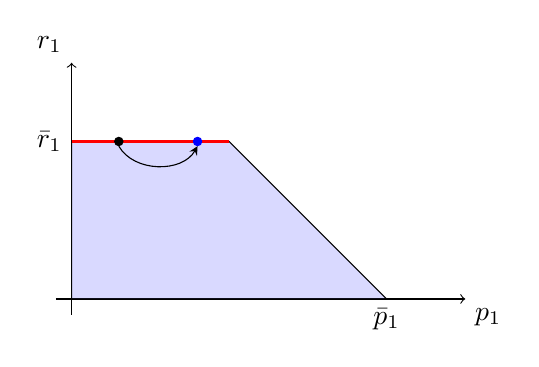
\begin{tikzpicture}[x=4cm,y=4cm]
                % X Axis
                \draw[black,->] (-0.05, 0) -- (1.25, 0);
                \node[below right] at (1.25, 0) {$p_{1}$};
                \node[below] at (1, 0) {$\bar{p}_{1}$};
                
                % Y axis
                \draw[black,->] (0, -0.05) -- (0, 0.75);
                \node[above left] at (0, 0.75) {$r_{1}$};
                \node[left] at (0, 0.5) {$\bar{r}_{1}$};
                
                % Domain of (p, r)
                \fill[blue!50!white, fill opacity=0.3] (0,0) -- (0, 0.5) -- (0.5, 0.5) -- (1,0) -- cycle;
                % Inactive constraints
                \draw[black] (0,0) -- (0, 0.5) -- (0.5,0.5) -- (1,0) -- cycle;
                % Active constraint (max reserve)
                \draw[red, line width=1pt] (0.0, 0.5) -- (0.5, 0.5);
                
                % Initial and feasible point
                \node[circle,draw=black, fill=black, inner sep=0pt,minimum size=3pt] (ppred) at (0.15, 0.5) {};
                \node[circle,draw=blue, fill=blue, inner sep=0pt,minimum size=3pt] (pfeas) at (0.4, 0.5) {};
                \draw[-stealth] (ppred.south) to [out=-60,in=-120] (pfeas.south);
            \end{tikzpicture}
            }
        \hfill
        \resizebox{0.45\columnwidth}{!}{
            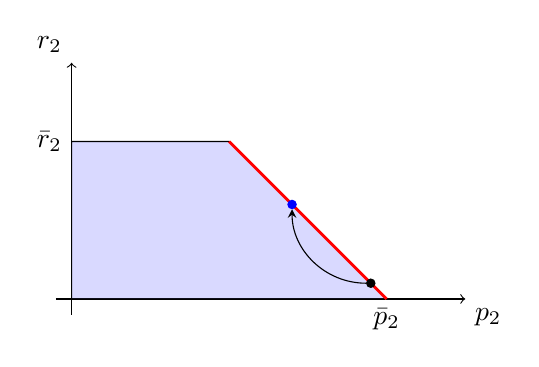
\begin{tikzpicture}[x=4cm,y=4cm]
                % X Axis
                \draw[black,->] (-0.05, 0) -- (1.25, 0);
                \node[below right] at (1.25, 0) {$p_{2}$};
                \node[below] at (1, 0) {$\bar{p}_{2}$};
                
                % Y axis
                \draw[black,->] (0, -0.05) -- (0, 0.75);
                \node[above left] at (0, 0.75) {$r_{2}$};
                \node[left] at (0, 0.5) {$\bar{r}_{2}$};
                
                % Domain of (p, r)
                \fill[blue!50!white, fill opacity=0.3] (0,0) -- (0, 0.5) -- (0.5, 0.5) -- (1,0) -- cycle;
                % Inactive constraints
                \draw[black] (0,0) -- (0, 0.5) -- (0.5, 0.5) -- (1,0) -- cycle;
                % Active constraint
                \draw[red, line width=1pt] (0.5, 0.5) -- (1.0, 0.0);
                
                % Initial and feasible point
                \node[circle,draw=black, fill=black, inner sep=0pt,minimum size=3pt] (ppred) at (0.95, 0.05) {};
                \node[circle,draw=blue, fill=blue, inner sep=0pt,minimum size=3pt] (pfeas) at (0.7, 0.3) {};
                \draw[-stealth] (ppred.west) to [out=180,in=-90] (pfeas.south);
            \end{tikzpicture}
            }
        \caption{Illustration of the reserve feasibility layer for $\mathbf{\bar{p}} {=} (1, 1)$, $\mathbf{\bar{r}}{=}(0.5, 0.5)$, $D {=} 1.1$, $R{=}0.8$ and the initial prediction $\pg {=} (0.15, 0.95)$. The recovered feasible dispatch is $\mathbf{\tilde{p}} {=} (0.4, 0.7)$.
        Top: effect of the layer in the $(p_{1}, p_{2})$ space.
        Bottom: effect of the layer on each generator (individually). The active constraint is shown in red. Generator $1$ is in $\mathcal{G}^{\uparrow}$ and generator 2 is in $\mathcal{G}^{\downarrow}$.}
        \label{fig:feasibility_recovery:reserve}
    \end{figure}
    

\subsection{End-to-end Feasible Training}
\label{sec:layers:end-to-end}

The repair layers are combined with a Deep Neural Network (DNN)
architecture to provide an end-to-end feasible ML model, i.e., a
differentiable architecture that is guaranteed to output a feasible
solution to Problem \eqref{eq:DCOPF} (if and only if one exists).  The
resulting architecture is illustrated in Figure
\ref{fig:end2end:architecture_detailed}.  The proxy takes as input the
vector of nodal demand $\pd$.  The DNN architecture consists of
fully-connected layers with ReLU activation, and a final layer with
sigmoid activations to enforce bound constraints on $\pg$.  Namely,
the last layer outputs $\mathbf{z} \in [0, 1]^{n}$, and
$\mathbf{\tilde{p}} = \mathbf{z} \cdot \pgmax$ satisfies constraints
\eqref{eq:DCOPF:dispatch_bounds}.  Then, this initial prediction
$\mathbf{\tilde{p}}$ is fed to the repair layers that restore the
feasibility of the power balance and reserve requirements.  The final
prediction $\mathbf{\hat{p}}$ is feasible for Problem
\eqref{eq:DCOPF}.
    
\begin{figure}[!t]
        \centering
        \includegraphics[width=\columnwidth]{images/architectures/FFR_v2.png}
        \caption{The Proposed End-To-End Feasible Architecture.}
        \label{fig:end2end:architecture_detailed}
    \end{figure}

The power balance and reserve feasibility layers only require
elementary arithmetic and logical operations, all of which are
supported by mainstream ML libraries like PyTorch and TensorFlow.
Therefore, it can be implemented as a layer of a generic artificial
neural network model trained with back-propagation.  Indeed, these
layers are differentiable almost everywhere with informative
(sub)gradients.  Finally, the proposed feasibility layers can be used
as a stand-alone, post-processing step to restore feasibility of any
dispatch vector that satisfies generation bounds.  This can be used
for instance to build fast heuristics with feasibility guarantees.
